\section{Contexto de trabajo}

Actualmente vivimos en un entorno que dominado por la tecnología. Día a día se desarrollan nuevas herramientas con el fin de ayudar al ser humano a realizar tareas de una forma más fácil y eficiente, como los HMD (Head-mounted Display)\cite{B15}.


Por otro lado también nos encontramos en una época donde el diseño es un área de gran importancia en cualquier sector del mercado, por ejemplo, un buen diseño web en un sitio es fundamental lograr que un producto se logre vender o difundir, un buen diseño gráfico en campañas de marketing asegura más clientes; de igual forma nos encontramos con el diseño de interiores. Para ésta última área se suelen contratar diseñadores de interiores profesionales para lograr que los espacios interiores de un inmueble consigan tal armonía que mejoren la calidad de vida de quienes lo habitan y además generen un impacto en las personas que usan éstas habitaciones.\par
El diseño de interiores profesional no sigue un proceso estandarizado, sin embargo a nivel general podemos ubicar las siguientes etapas:

\begin{itemize}
	\item El cliente acude con un diseñador de interiores profesional, quien acude al domicilio para conocer las condiciones del inmueble y conocer las necesidades y presupuesto del cliente.
	\item Conociendo estos dos puntos el diseñador hace un análisis de viabilidad que se compone de un análisis presupuestal y la definición del alcance del diseño.
	\item El diseñador le muestra esta información al cliente para que la apruebe, en caso de no ser así, el proyecto es considerado como no viable.
	\item De ser viable el diseñador de interiores genera un calendario previo de actividades donde programa el cumplimiento de los requerimientos del cliente en determinadas fechas.
	\item Si el cliente aprueba la propuesta de calendario, el diseñador se dispone a realizar el \textbf{proceso de propuesta de diseño de interiores} con el objetivo de mostrarle al cliente el resultado final previo de la obra antes de que sea realizada, esta propuesta puede mostrarse de varias formas como fotografías con fotomontajes, una explicación verbal con fotografías de apoyo (de muebles o habitaciones ya decoradas) o un modelado tridimensional del resultado de la obra; se suele usar un modelado tridimensional pues es lo más cercano a la realidad que se le puede mostrar al cliente. Si el cliente no aprueba la propuesta de calendario, se debe volver a realizar el análisis de viabilidad para ajustarse a las necesidades y presupuesto del cliente.
	\item El diseñador le muestra la propuesta de diseño al cliente y si esta es aceptada, se inicia el desarrollo de la obra con base en las fechas establecidas.
	\item Finalmente el diseñador entrega la obra al cliente y termina el proceso de diseño de interiores.
\end{itemize}

El proceso completo anteriormente descrito se puede observar en la figura 1.1 a través de un diagrama de proceso de negocio, en las figuras 1.2 y 1.3 se muestra el diagrama segmentado para una mejor lectura del mismo, y en la figura 1.4 puede observar el \textbf{proceso de propuesta de diseño de interiores}.\par
Teniendo a la mano una gran diversidad de herramientas tecnológicas, podemos usar estos elementos para lograr que el diseño de interiores sea más sencillo y rápido, tanto para un diseñador de interiores que vaya a realizar una obra para algún cliente, como para alguien que desee diseñar o rediseñar su propio inmueble.
\newpage

\begin{figure}[!htbp]
	\centering
	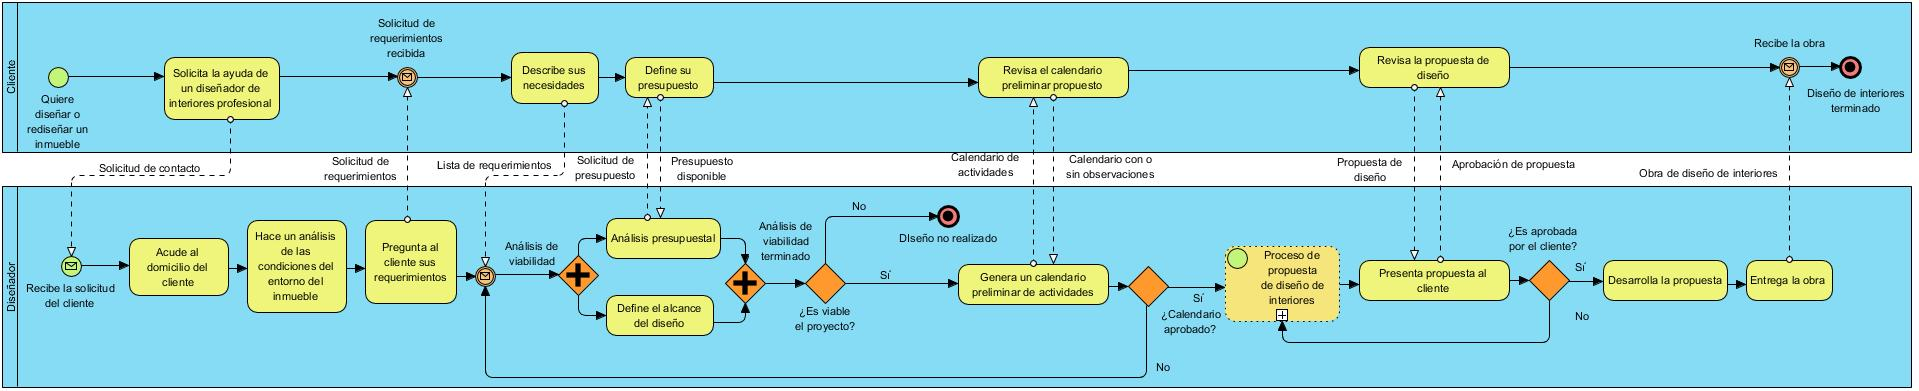
\includegraphics[width=20cm,angle=270,origin=c]{imagenes/marcoteorico/bpmn/proceso_full.jpg}
	\caption{Modelo del proceso de diseño de interiores (Completo).}
	\label{fig:bpmn_antes}
\end{figure}
\newpage

\begin{figure}[!htbp]
	\centering
	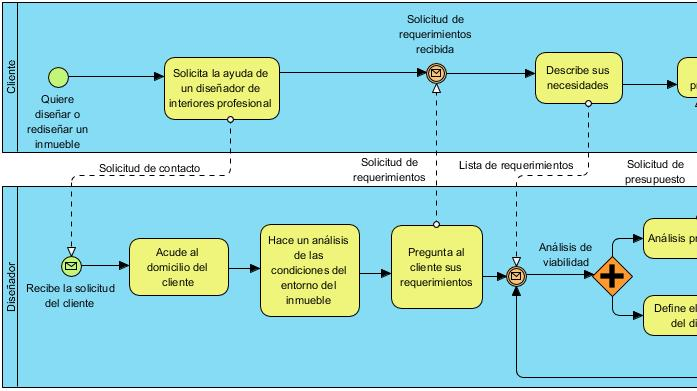
\includegraphics[width=19cm,angle=270,origin=c]{imagenes/marcoteorico/bpmn/proceso_01_01.jpg}
	\caption{Modelo del proceso de diseño de interiores (Segmento I).}
	\label{fig:bpmn_antes}
\end{figure}
\newpage

\begin{figure}[!htbp]
	\centering
	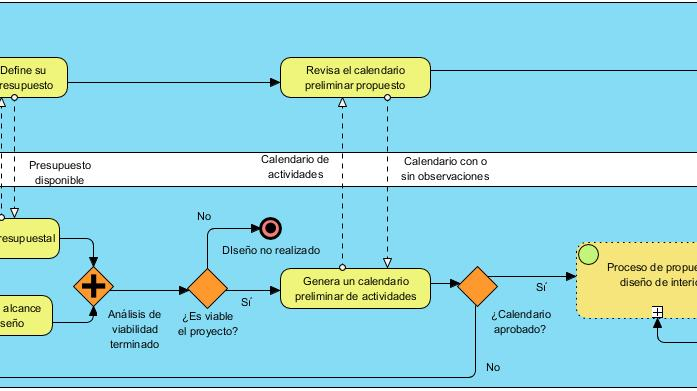
\includegraphics[width=19cm,angle=270,origin=c]{imagenes/marcoteorico/bpmn/proceso_02_01.jpg}
	\caption{Modelo del proceso de diseño de interiores (Segmento II).}
	\label{fig:bpmn_antes}
\end{figure}
\newpage

\begin{figure}[!htbp]
	\centering
	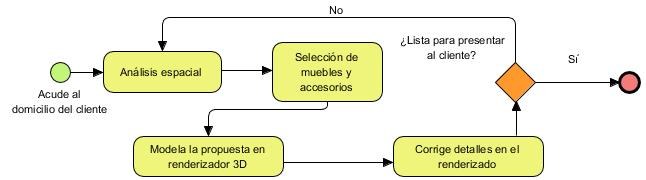
\includegraphics[width=16cm]{imagenes/marcoteorico/bpmn/subproceso.jpg}
	\caption{Subproceso de propuesta de diseño de interiores.}
	\label{fig:subproceso}
\end{figure}
\newpage